\documentclass[11pt]{article}

\newcommand{\cnum}{CM146}
\newcommand{\ced}{Winter 2018}
\newcommand{\ctitle}[3]{\title{\vspace{-0.5in}\cnum, \ced\\Problem Set #1: #2}}

\newcommand{\solution}[1]{{{\color{blue}{\bf Solution:} {#1}}}}
\usepackage[usenames,dvipsnames,svgnames,table,hyperref]{xcolor}
\usepackage{amsmath, listings, graphicx}
\renewcommand*{\theenumi}{\alph{enumi}}
\renewcommand*\labelenumi{(\theenumi)}
\renewcommand*{\theenumii}{\roman{enumii}}
\renewcommand*\labelenumii{\theenumii.}
\graphicspath{{images/}}

\begin{document}
\ctitle{xx}{yy}
\author{}
\date{}
\maketitle
\vspace{-0.75in}

\section{Problem 1}
\begin{enumerate}
\item Problem 1

\solution{}
\[
	\frac{\partial y}{\partial x} = (\sin{z}) (e^{-x} - xe^{-x})
\]
\vspace{10cm}
\end{enumerate}

\newpage
\section{Problem 2}

\begin{enumerate}
\item Problem 2a
\solution{}
$$
\begin{pmatrix}
1 & 3
\end{pmatrix}
\begin{pmatrix}
2 \\
3
\end{pmatrix}
= 
\begin{pmatrix}
11
\end{pmatrix}
$$

\item Problem 2b
\solution{}
$$
\begin{pmatrix}
2 & 4 \\
1 & 3
\end{pmatrix}
\begin{pmatrix}
1 \\
3
\end{pmatrix}
=
\begin{pmatrix}
14 \\
10
\end{pmatrix}
$$

\item Problem 2c
\solution{}

Yes, the matrix X is invertible since it has a non-zero determinant \break
$$
\begin{vmatrix}
2 & 4 \\
1 & 3
\end{vmatrix}
= 6 - 4 = 2 
$$
$$
X^{-1} = \frac{1}{2}
\begin{pmatrix}
3 & -4 \\
-1 & 2
\end{pmatrix}
$$

\item Problem 2d
\solution{}
The rank of X is 2 (since it is invertible)
\end{enumerate}

\newpage

\section{Problem 3}
\begin{enumerate}

\item Problem 3a
\solution{}
$$
Sample\quad Mean = \frac{1 + 1 + 0 + 1 + 0}{5} = \frac{3}{5} = 0.6
$$


\item Problem 3b
\solution{}
TODO!!!!

\item Problem 3c
\solution{}
Probability of observing this pattern is:
$$
\frac{1}{2^5} = \frac{1}{32}
$$

\item Problem 3d
\solution{}
Let the probability 
$$
P(X_{i} = 0) = p
$$
$$
P(X_{i} = 1) = (1 - p)
$$
Probability of pattern (since all events are independent):
$$
X = \frac{1}{1-p} \cdot \frac{1}{1-p} \cdot \frac{1}{p} \cdot \frac{1}{1-p} \cdot \frac{1}{p} = \frac{1}{p^2 - 3p^3 + 3p^4 - p^5}
$$
Taking the derivative of the above equation, and setting it to zero gives us the following equation
$$
- {(p-1)}^2 (5p - 2) = 0
$$
$$
\rightarrow p = \frac{2}{5}
$$
$$
\rightarrow P(X_{i} = 1) = \frac{3}{5}
$$

\item Problem 3e
\solution{}
$$
P(X = T | Y = b) = \frac{0.1}{0.1 + 0.15} = \frac{0.1}{0.25} = \frac{2}{5}
$$
\end{enumerate}

\newpage
\section{Problem 4}
\begin{enumerate}

\item Problem 4a
\solution{}
False

\item Problem 4b
\solution{}
True

\item Problem 4c
\solution{}
False

\item Problem 4d
\solution{}
False

\item Problem 4e
\solution{}
True

\end{enumerate}

\newpage

\section{Problem 5}

(a) - (v) \newline
(b) - (iv) \newline
(c) - (ii) \newline
(d) - (i) \newline
(e) - (iii) 

\newpage
\section{Problem 6}
\begin{enumerate}
\item Problem 6a
\solution{}
Mean of a Bernoulli random variable = p \newline
Variance of a Bernoulli random variable = p(1 - p)

\item Problem 6b
\solution{} \newline
$$var(X) = \sigma ^ 2$$
$$var(2X) = 4 \sigma ^ 2$$
$$var(X + 2) =  \sigma ^ 2$$
\end{enumerate}

\newpage
\section{Problem 7}
\begin{enumerate}
\item Problem 7a (i)
\solution{}
Both f(n) = O(g(n)) and g(n) = O(f(n)) are true

\item Problem 7a (ii)
\solution{}
f(n) = O(g(n))

\item Problem 7a (iii)
\solution{}
f(n) = O(g(n))

\item Problem 7b
\solution{}
\begin{lstlisting}
findTransition(Array a, startIndex, endIndex):
	middle = (startIndex + endIndex ) / 2
	if(a[middle] is 0 and a[middle + 1] is a 1):
		// transition point found
		return middle
	else if (a[middle] and a[middle] are both 0):
		// both elements in the center are 0, so search in 
			// the right half of the array
		return findTransition(a, middle, endIndex)
		
	else: // both elements at a[middle] and a[middle + 1] 
			// are 1, so search in left half of the array
		return findTransition(a, 0, middle)
\end{lstlisting}
\begin{verbatim}		
Correctness:
	Suppose the transition from 0s to 1s happens at index i (i > n/2), where n 
	is the number of elements in the array. Since the transition happens in the 
	second half of the array, all elements to the left of the middle index are 0s, 
	and we only need to search the right half of the array. On the recursive call, 
	the problem remains the same but is a smaller problem. Similarly, it can be 
	shown that the algorithm will always examine the correct index if i < n/2. If 
	the transition happens in the dead center, then this will be found on the first
	call and the result returned. Hence, the algorithm is correct.

Runtime:
	At every recursive call, the problem size is reduced by half. This can 
	be given by the recurrence relation:
		T(n) = T(n/2) + O(1)
	The solution to this recurrence relation is an algorithm of O(log n) time. 
\end{verbatim}



\end{enumerate}

\newpage
\section{Problem 8}
\begin{enumerate}
\item Problem 8a
\solution{}
$$
	E[XY] = \sum_{x,y} xy p_{X,Y}(x,y)
$$
Since X, Y are independent: 
$$
	E[XY] = \sum_{x,y} xy p_{X}(x) p_{Y}(y) \qquad $$
$$
	E[XY] = \sum_{x} x p_{X}(x) \sum_{y} y p_{Y}(y)
$$
$$
	E[XY] = E[X]E[Y]
$$

\item Problem 8b (i)
\solution{}
TODO!!!
\item Problem 8b (ii)
\solution{}
TODO!!!
\end{enumerate}

\newpage
\section{Problem 9}
\subsection{9a}
\begin{enumerate}
\item Problem 9a (i)
\solution{}
\newline
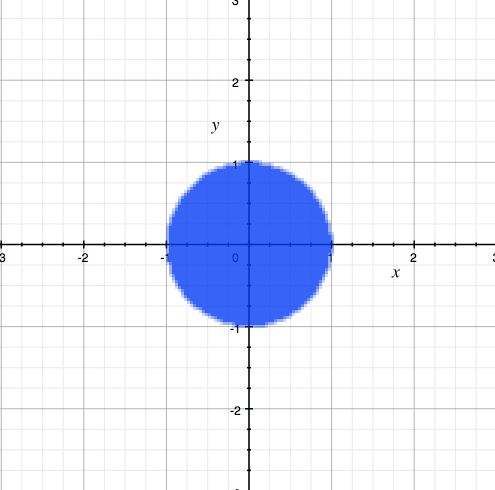
\includegraphics[scale=0.4]{9a(i)}

\iffalse
\item Problem 9a (ii)
\solution{}
\newline
TODO!!!
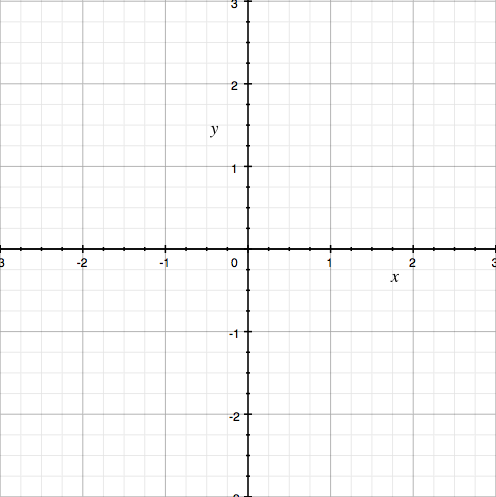
\includegraphics[scale=0.4]{9a(ii)}
\fi

\item Problem 9a (iii)
\solution{}
\newline
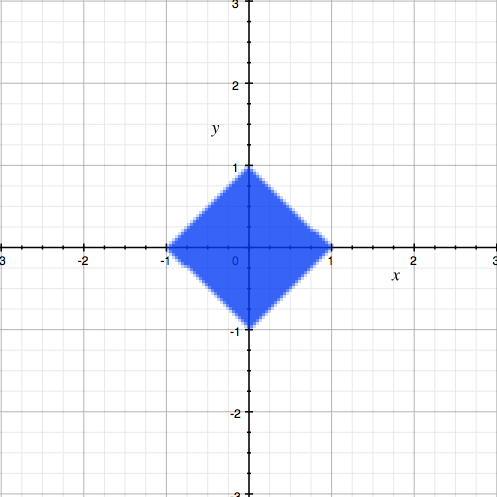
\includegraphics[scale=0.4]{9a(iii)}

\item Problem 9a (iv)
\solution{}
\newline
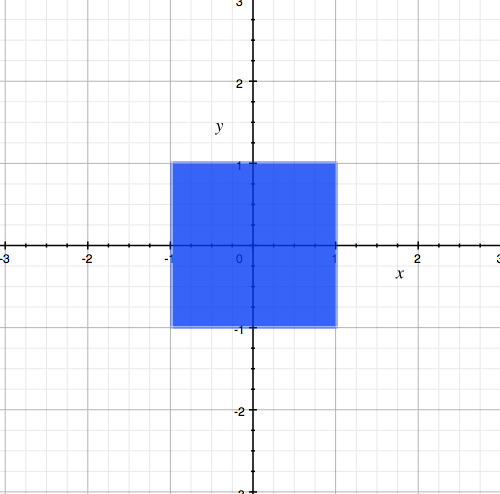
\includegraphics[scale=0.4]{9a(iv)}

\end{enumerate}

\subsection{9b}
\begin{enumerate}
\item 9b (i)
\solution{}
The eigenvector $\vec{v}$ of a square matrix, $A$ is a vector such that $$ A\vec{v} = \lambda \vec{v}$$
The scalar $\lambda$ is called an eigenvalue of the square matrix.

\item 9b (ii)
\solution{}
The eigenvalues can be found by setting the determinant of the matrix $ A - \lambda I$ equal to 0
$$
\begin{vmatrix}
2 - \lambda & 1 \\
1 & 2 - \lambda
\end{vmatrix}
 = 0
$$
$$
(2 - \lambda)^2 - 1 = 0
$$
$$
\lambda ^ 2 - 4 \lambda + 3 = 0
$$
$$
(\lambda - 3)(\lambda - 1) = 0
$$
$$
\Rightarrow \lambda = 3, 1
$$
To find the eigenvectors, we find a vector such that $(A - \lambda I)\vec{v} = 0 $
\newline
For $\lambda = 3$
$$
\begin{pmatrix}
-1 & 1 \\
1 & -1 
\end{pmatrix}
\vec{x} = 0
$$
$$
\vec{x} = 
\begin{bmatrix}
1 \\
1
\end{bmatrix}
$$
\newline
For $\lambda = 1$
$$
\begin{pmatrix}
1 & 1 \\
1 & 1
\end{pmatrix}
\vec{x} = 0
$$
$$
\vec{x} = 
\begin{bmatrix}
1 \\
-1
\end{bmatrix}
$$

\item Problem 9b (iii)
\solution{}


\end{enumerate}


\end{document}
